\chapter{Računalni vid}

Računalni vid \engl{computer vision} je grana računarske znanosti, točnije područja umjetne inteligencije, koja pokušava omogućiti računalima da interpretiraju  vizualne podatke te iz njih izvuku nove informacije. To je zasigurno jedno od trenutno najuzbudljivijih i najbrže rastućih područja umjetne inteligencije, čije primjene sežu od automatskog označavanja ljudi na slikama koje objavljujemo na Instagramu i Facebooku, sve do autonomne vožnje i primjena u medicini i znanosti. Ovo područje danas doživljava svoju renesansu, u velikom dijelu zbog pojave algoritama baziranih na dubokom učenju i napretka u računalnim resursima. No ne treba zaboraviti da je računalni vid UI-potpun problem, te da je put koji smo morali prijeći da dođemo do današnjih uspjeha bio sve osim lagan.\\ \\
U ovom poglavlju dati ću osnovu podjelu područja računalnog vida te se kratko osvrnuti na njihovu praktičnu primjenu.
\section{Podjela računalnog vida}

Područje računalnog vida obuhvaća mnoga i raznolika područja. Analiza pokreta u video snimkama, detekcija objekata, rekonstrukcija 3D scene iz 2D slike su samo neki od primjera raznovrsnosti računalnog vida. Nas zanima jedno konkretno područje - detekcija objekata u 2D slikama. Glavni zadatak tog područja je, kako mu samo ime i kaže, izvući razne informacije o položaju objekata unutar slike. Ovisno o vrsti informacije, ovo područje dalje možemo podijeliti na klasifikaciju, lokalizaciju, detekciju, semantičku segmentaciju te segmentaciju instanci.

\subsection{Klasifikacija}
Najjednostavnija varijanta detekcije objekata, klasifikacija \engl{classification}, nastoji zadanu sliku svrstati u neku od predefiniranih klasa. Na primjer, ukoliko algoritmu za klasifikaciju kao ulaz predamo sliku na kojoj se nalazi mačić koji sjedi na livadu, mogli bismo očekivati da će algoritam slici pridijeliti oznaku \textit{mačka}, iako su na slici prisutni i drugi elementi poput trave, oblaka ili sunca. Povećanjem broja klasa težina problema se povećava. 

\subsection{Lokalizacija}
Sljedeći, nešto napredniji korak je lokalizacija \engl{localization}, odnosno utvrđivanje točne lokacije \textbf{jednog} objekta na slici. Na već spomenutom primjeru s mačićem na livadi, cilj bi nam bio označiti točnu lokaciju mačića u slici, najčešće crtanjem pravokutnika oko njegove lokacije.

\subsection{Detekcija}
Detekcija \engl{detection} je u svojoj osnovi vrlo slična lokalizaciji, samo što za razliku od lokalizacije, koja utvrđuje lokaciju jednog objekta na slici, detekcija utvrđuje točnu lokaciju svih instanci objekata za slici (za koje postoje zadane klase).  Česta primjena ove vrste detekcije objekata je u autonomnoj vožnji, gdje je za upravljački softver vrlo važno da zna točnu lokaciju ostalih vozila, pješaka itd., kako bi mogao donijeti ispravnu odluku o upravljanju vozilom.

\subsection{Semantička segmentacija}
Semantička segmentacija \engl{semantic segmentation} ide korak dalje, te za svaki piksel u slici nastoji odrediti kojoj klasi pripada. Ovaj problem je znatno složeniji nego prethodna tri, jer zahtjeva značajnije razumijevanje semantike slike u odnosu na prethodne. Ova vrsta detekcije također ima primjene u sustavu za autonomnu vožnju, ali i u drugim područjima, od kojih valja istaknuti primjenu u području medicinskih slika. Ovo je pristup koji nas najviše zanima i koji ćemo pobliže istražiti u nastavku ovog rada.

\subsection{Segmentacija instanci }
Segmentacija instanci \engl{instance segmentation} je složeniji oblik semantičke segmentacije, gdje se svaki piksel u slici nastoji pridijeliti točno jednoj \textbf{instanci} određene klase. Dakle, ako na slici imamo tri mačića, pikseli kojima su oni prikazani na slici pripadat će klasi mačić, ali model će također znati razlikovati pripada li određeni piksel mačiću 1, 2 ili 3.


\begin{figure}[htb]
\centering
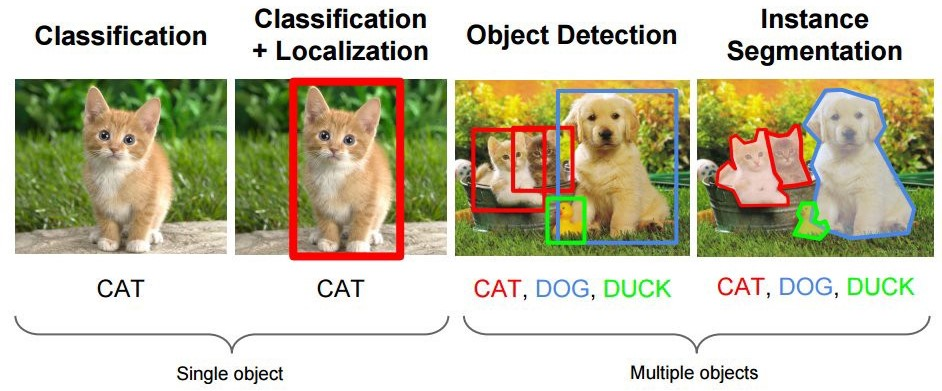
\includegraphics[width=14cm]{slike/object_detection.jpeg}
\caption{Usporedba načina detekcije \citep{objectDetectionMethodsImg}}
\label{fig:fer-logo}
\end{figure}
\textbf{}

\noindent Iako je rješavanje svih navedenih problema gotovo trivijalno za ljude, oni računalima predstavljaju velik izazov. Stoga ćemo u sljedećim poglavljima detaljnije pogledati jedan pristup koji se do sad pokazao najboljim - duboko učenje.
